\begin{itemize}
    \item Análisis del problema
        \begin{itemize}
        
            \item Descripción general:
            El sistema de monitoreo con alarmas supervisa continuamente una variable física y clasifica su valor en tres niveles operativos: Normal, Advertencia y Crítico. Para cada nivel se activan indicadores visuales y/o sonoros diferenciados. Se implementa histéresis para evitar oscilaciones inestables en los umbrales de transición.

        \end{itemize} 

    \item Identificación de Entradas y Salidas
        \begin{itemize}
            
            \item Entradas:
                \begin{itemize}
                    \item  Sensor de temperatura (señal analógica o digital).

                    \item Botón de silencio de alarma (opcional).                   
                \end{itemize}
            
            \item Salidas:
                \begin{itemize}
                    \item  LED verde: estado Normal.
                    
                    \item LED amarillo: estado Advertencia.    
                    \item LED rojo: estado Crítico. 

                    \item Buzzer: alarma sonora en Advertencia y Crítico.
                    
                \end{itemize}

    \item Restricciones técnicas
        \begin{itemize}
            \item Los umbrales deben ser configurables mediante constantes.

            \item Implementación obligatoria de histéresis para evitar inestabilidad en los límites.
            
            \item El sistema debe funcionar en ciclo continuo con temporización no bloqueante.
            
            \item La lectura del sensor debe ser promediada para reducir ruido.
            
        \end{itemize}
       
    \item Definición de umbrales y variables:

    En la Tabla~\ref{tab:Tabla_1_R2}, se observa la definición de las variables con sus respectivas descripciones y justificación. Reconocer las variables a utilizar sera de ayuda a la hora de realizar el código.

    

\begin{table}[!ht]
\centering
\caption{Definición de Umbrales y Variables}
\label{tab:Tabla_1_R2}
\footnotesize
\setlength{\tabcolsep}{3pt}
\renewcommand{\arraystretch}{1.3}
    \begin{tabularx}{\columnwidth}{|p{3.2cm}|p{2cm}|X|}

        \hline
        \textbf{Variable} & \textbf{Valor} & \textbf{Descripción} \\ 

        \hline UMBRAL\_ADVERTENCIA & const = 30°C & Umbral para activar advertencia \\ 

        \hline UMBRAL\_CRITICO & const = 40°C & Umbral para nivel crítico \\ 

        \hline HISTERESIS & const = 2°C & Margen para evitar fluctuaciones \\ 

        \hline temperaturaActual & float & Valor del sensor en °C \\ 

        \hline estadoActual & enum & NORMAL, ADVERTENCIA, CRÍTICO \\ 
    
        \hline tiempoUltimaLectura & unsigned long & Timestamp de la lectura \\ 
        
        \hline
    \end{tabularx}
\end{table}

    \item Flujograma del Sistema

    El algoritmo, que se observa como Algoritmo ~\ref{alg:control_temp},
    funciona en ciclo continuo, e implementa un sistema de monitoreo de temperatura basado en una máquina de estados con tres niveles: NORMAL, ADVERTENCIA y CRÍTICO. Cada 500 ms se realiza una nueva lectura del sensor, se calcula la temperatura y se determina el estado del sistema aplicando histéresis. En función del estado, se activan los indicadores correspondientes.
    
    

\begin{algorithm}[t]
\caption{Control de Temperatura con Histéresis}
\label{alg:control_temp}
\begin{algorithmic}[1]

\Statex \textbf{INICIO}
\State Inicializar pines, LCD, sensor
\State $\text{estadoActual} \gets \text{NORMAL}$

\Loop \ \textbf{PRINCIPAL} (cada 500 ms)
    \State $\text{temperaturaActual} \gets \text{leerSensor}()$
    
    \If{$\text{estadoActual} = \text{NORMAL}$}
        \If{$\text{temperaturaActual} \geq \text{UMBRAL\_ADVERTENCIA}$}
            \State $\text{estadoActual} \gets \text{ADVERTENCIA}$
        \EndIf

    \ElsIf{$\text{estadoActual} = \text{ADVERTENCIA}$}
        \If{$\text{temperaturaActual} \geq \text{UMBRAL\_CRITICO}$}
            \State $\text{estadoActual} \gets \text{CRITICO}$
        \ElsIf{$\text{temperaturaActual} < (\text{UMBRAL\_ADVERTENCIA} - \text{HISTERESIS})$}
            \State $\text{estadoActual} \gets \text{NORMAL}$
        \EndIf

    \ElsIf{$\text{estadoActual} = \text{CRITICO}$}
        \If{$\text{temperaturaActual} < (\text{UMBRAL\_CRITICO} - \text{HISTERESIS})$}
            \State $\text{estadoActual} \gets \text{ADVERTENCIA}$
        \EndIf
    \EndIf

    \State actualizarIndicadores($\text{estadoActual}$)
    \State mostrarEnLCD($\text{temperaturaActual, estadoActual}$)
\EndLoop
\Statex \textbf{FIN}

\end{algorithmic}
\end{algorithm}

    \item Justificación técnica del microcontrolador
        \begin{itemize}
            \item Microcontrolador Seleccionado: Arduino UNO (ATmega328P)

            El mismo microcontrolador del reto anterior es suficiente para este segundo reto.  Para usar el DHT21, se requiere únicamente un pin digital con protocolo one-wire.

            \item Análisis de Pines Requeridos:

            En la Tabla~\ref{tab:Tabla_2_R2}, se observan los pines solicitados para el correcto funcionamiento del programa.

            
\begin{table}[ht]
\caption{Análisis de Pines Requeridos (Sistema de Monitoreo)}
\label{tab:Tabla_2_R2}
\centering
\renewcommand{\arraystretch}{1.3}
\begin{tabularx}{\columnwidth}{X p{2.0cm} p{2.0cm}}
\toprule
\textbf{Componente} & \textbf{Pin} & \textbf{Tipo} \\
\midrule
Sensor NTC / DHT21 & A0 o D2 & Analógico / Digital \\
LED verde & D9 & Digital OUTPUT \\
LED amarillo & D10 & Digital OUTPUT \\
LED rojo & D11 & Digital OUTPUT \\
Buzzer & D8 & Digital OUTPUT \\

\midrule
\textbf{Total} & \textbf{6 pines} & --- \\
\bottomrule
\end{tabularx}
\end{table}

            \item Componentes auxiliares

            El sistema emplea como elemento principal de medición un sensor de temperatura DHT21. La visualización de la información se realiza mediante monitor serial en el Arduino IDE, lo que optimiza el uso de pines del microcontrolador.
            
            Para la señalización del estado del sistema se utilizan tres LEDs de 5 mm (verde, amarillo y rojo) de 20 mA, cada uno con su respectiva resistencia limitadora de 220 ohms para protección. Además, se integra un buzzer activo de 5 V y aproximadamente 85 dB que funciona como alarma sonora en condiciones críticas, reforzando la advertencia al usuario.

            \item Esquema de conexión 

            En la Figura \ref{fig:Imagen_1R2} se observa el diagrama de conexión correspondiente al funcionamiento de este circuito, desarrollado a través del programa de circuitado. A continuación se mencionan las conexiones realizadas:
            \begin{itemize}
                \item Sensor DHT21: D2 → pin DATA (resistencia pull-up 10k ohms entre DATA y VCC), VCC a 5V, GND a GND
                \item LED verde: D9 → 220 ohms → LED → GND
                \item LED amarillo: D10 → 220 ohms → LED → GND
                \item LED rojo: D11 → 220 ohms → LED → GND
                \item Buzzer: D8 → buzzer (+) → GND
            \end{itemize}
            \textit{EasyEDA}.
                  \begin{figure}[h]
                  \centering
                  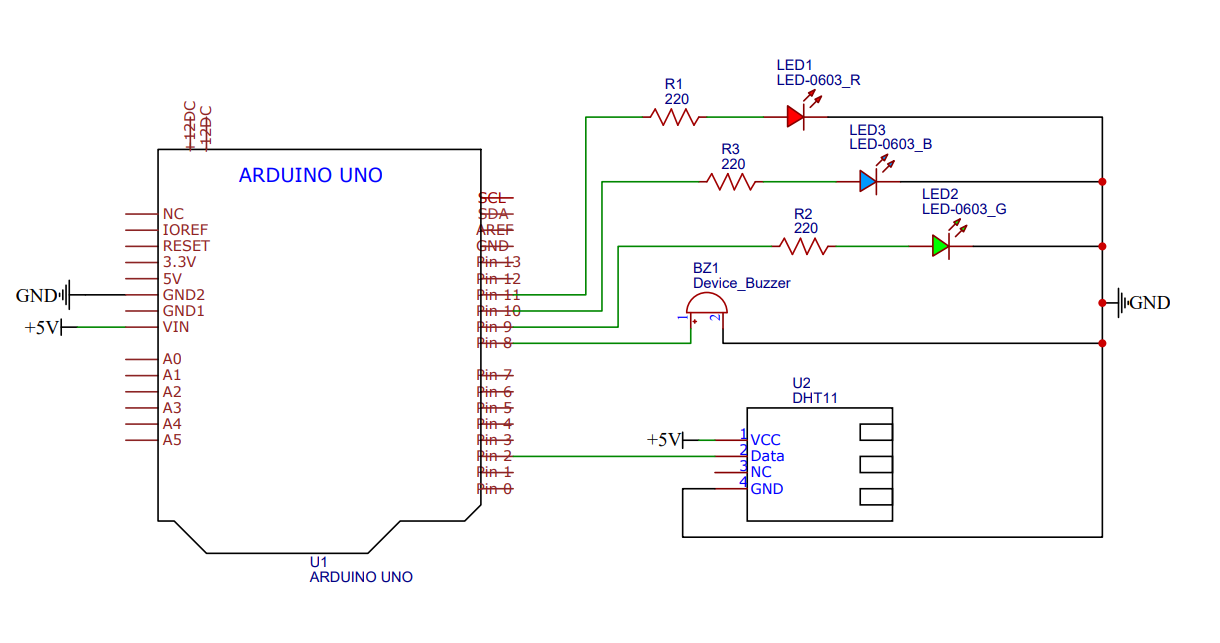
\includegraphics[width=\columnwidth]{images/Imagen_1R2.png}
                  \caption{Esquemático de Conexión Reto 2}
                  \label{fig:Imagen_1R2}
                  \end{figure}
            
        \end{itemize}

    \item Código Documentado

    El código propuesto documentado se encuentra registrado a continuación:
    \begin{lstlisting}[caption={Sistema de Monitoreo de Temperatura con DHT11}, label={lst:monitoreo-temperatura}]
#include <DHT.h>

// --- Pines ---
const int PIN_SENSOR       = 2;
const int PIN_LED_VERDE    = 9;
const int PIN_LED_AMARILLO = 10;
const int PIN_LED_ROJO     = 11;
const int PIN_BUZZER       = 8;

// --- Configuracion DHT11 ---
#define DHTTYPE DHT11
DHT dht(PIN_SENSOR, DHTTYPE);

// --- Umbrales de temperatura ---
const float UMBRAL_ADVERTENCIA = 30.0;  
const float UMBRAL_CRITICO     = 40.0;  
const float HISTERESIS         = 2.0;   

// --- Enumeracion de estados ---
enum EstadoSistema 
{ NORMAL, ADVERTENCIA, CRITICO };
EstadoSistema estadoActual = NORMAL;

// --- Variables de temporizacion ---
unsigned long tiempoUltimaLectura = 0;
const long    INTERVALO_LECTURA   = 2000;
unsigned long tiempoBuzzer        = 0;
bool          estadoBuzzer        = false;

float leerTemperatura() {
  float temp = dht.readTemperature();
  if (isnan(temp)) {
    Serial.println("Error al leer 
    el DHT11");
    return -999.0;
  }
  return temp;
}

void evaluarEstado(float temperatura) {
  if (temperatura == -999.0) return;
  switch (estadoActual) {
    case NORMAL:
      if (temperatura >= 
      UMBRAL_ADVERTENCIA)
        estadoActual = ADVERTENCIA;
      break;
    case ADVERTENCIA:
      if (temperatura >= UMBRAL_CRITICO)
        estadoActual = CRITICO;
      else if (temperatura < 
               UMBRAL_ADVERTENCIA 
               - HISTERESIS)
        estadoActual = NORMAL;
      break;
    case CRITICO:
      if (temperatura < UMBRAL_CRITICO 
      - HISTERESIS)
        estadoActual = ADVERTENCIA;
      break;
  }
}

void actualizarLEDs() {
  digitalWrite(PIN_LED_VERDE,
               estadoActual == NORMAL);
  digitalWrite(PIN_LED_AMARILLO,
               estadoActual == 
               ADVERTENCIA);
  digitalWrite(PIN_LED_ROJO,
               estadoActual == 
               CRITICO);
}

void gestionarBuzzer() {
  if (estadoActual == NORMAL) {
    noTone(PIN_BUZZER);
    return;
  }
  long intervalo = 
    (estadoActual == ADVERTENCIA)
    ? 1000 : 250;
  if ((millis() - tiempoBuzzer)
  >= intervalo) {
    tiempoBuzzer = millis();
    estadoBuzzer = !estadoBuzzer;
    if (estadoBuzzer)
      tone(PIN_BUZZER, 1500,
      intervalo / 2);
    else
      noTone(PIN_BUZZER);
  }
}

void setup() {
  Serial.begin(9600);
  dht.begin();
  pinMode(PIN_LED_VERDE,    OUTPUT);
  pinMode(PIN_LED_AMARILLO, OUTPUT);
  pinMode(PIN_LED_ROJO,     OUTPUT);
  pinMode(PIN_BUZZER,       OUTPUT);
  Serial.println("Sistema de 
  Monitoreo - Activo");
}

void loop() {
  unsigned long ahora = millis();
  if (ahora - tiempoUltimaLectura >= 
      INTERVALO_LECTURA) {
    tiempoUltimaLectura = ahora;
    float temperatura = leerTemperatura();
    evaluarEstado(temperatura);
    actualizarLEDs();
    Serial.print("T=");
    Serial.print(temperatura);
    Serial.print(" Estado=");
    Serial.println(estadoActual);
  }
  gestionarBuzzer();
}
\end{lstlisting}


    
    \end{itemize}  
\end{itemize}